\documentclass[11pt,letterpaper]{article}

%%%%%%%%%%%%%%%%%%%%%%%%%%%%%%                               
\pagestyle{plain}                                                      %%
%%%%%%%%%% EXACT 1in MARGINS %%%%%%%                                   %%
\setlength{\textwidth}{6.5in}     %%                                   %%
\setlength{\oddsidemargin}{0in}   %% (It is recommended that you       %%
\setlength{\evensidemargin}{0in}  %%  not change these parameters,     %%
\setlength{\textheight}{9.0in}    %%  at the risk of having your       %%
\setlength{\topmargin}{0in}       %%  proposal dismissed on the basis  %%
\setlength{\headheight}{0in}      %%  of incorrect formatting!!!)      %%
\setlength{\headsep}{0in}         %%                                   %%
\setlength{\footskip}{.5in}       %%                                   %%

%%%%%%%%%%%%%%%%%%%%%%%%%%%%%%%%%%%%                                     

\usepackage[pdftex]{graphicx}
\usepackage{color}
\usepackage{url}
\usepackage{tabularx}
\usepackage{tikz}

% From PPoPP
\usepackage{amsmath}
\usepackage{amsfonts}
%  \usepackage{graphicx}
  %  \usepackage{xspace}
\usepackage{verbatim}
%  \usepackage{listings}
\usepackage{multirow}
\usepackage{subfigure}
\usepackage{pdfpages}
%% % Tweak spacing to fit in page limit if needed
%% % ============================================
%% % gap between text and figs/tables:
%% \addtolength\textfloatsep{-0.2in}
%% % gap between figs/tables and other figs/tables
%% \addtolength\floatsep{-0.1in}
%% % gap between figure and caption
%% \addtolength\abovecaptionskip{-0.05in}
%% \addtolength\intextsep{0in}

\hyphenation{ }

\setlength{\parindent}{0.5cm}

\newif\ifdraft
% comment out the next line to turn off comments
% \drafttrue
\drafttrue

\ifdraft
\definecolor{darkgreen}{rgb}{0,0.5,0}
\newcommand{\manish}[1]{{\it \color{red} #1 -Manish}}
\newcommand{\hasan}[1]{{\it \color{darkgreen} #1 -Hasan }}
\definecolor{orange}{rgb}{0.7,0.5,0.0}
\newcommand{\klasky}[1]{{\textcolor{orange} #1 -Scott }}
  % Red star denotes items that need further work or discussio
\newcommand{\TODO}[1]{\textcolor{red}{ TO DO: #1 }}
\newcommand{\ALT}[1]{{\color{red} #1 - {\bf Alternate Text}}}
\else
\definecolor{darkgreen}{rgb}{0,0.5,0}
\newcommand{\manish}[1]{}
\definecolor{orange}{rgb}{0.7,0.5,0.0}
% Red star denotes items that need further work or discussion
\newcommand{\TODO}[1]{}
\newcommand{\klasky}[1]{}
\newcommand{\hasan}[1]{}
\newcommand{\ALT}[1]{}}
\fi

%  \newcommand{\ititle}{\textsc{\textbf{HESK}}}
\newcommand{\ititle}{\textsc{HESK}}
\newcommand{\insitu}{\textit{in situ }}

\let\oldenumerate\enumerate
\renewcommand{\enumerate}{
  \oldenumerate
  \setlength{\itemsep}{1pt}
  \setlength{\parskip}{0pt}
  \setlength{\parsep}{0pt}
}

% A definition we do not want the reader to forget
\newcommand{\defn}[1] {\textbf{\textit{#1}}}

\definecolor{teal}{rgb}{0.06,0.3,0.3}
\definecolor{maroon}{rgb}{0.5,0.0,0.25}
\definecolor{darkblue}{rgb}{0.0,0.2,0.75}
\definecolor{darkred}{rgb}{0.7,0.0,0.0}
\definecolor{darkgreen2}{rgb}{0,0.35,0}

\newcommand*\circled[1]{\tikz[baseline=(char.base)]{
    \node[shape=circle,draw,inner sep=2pt] (char) {#1};}}


\begin{document}
\begin{comment}
  \noindent
  \textbf{Pre-proposal Cover Sheet}
  \newline
  \vskip .1in
  Storage Systems and Input/Output for Extreme Scale Science 
  Scale 2 (LAB 14-1043)

  \vskip .3in

  \noindent
  \textbf{Project title:}
  \vskip .1in
  Hierarchal Extreme Scale Knowledge Management


  \vskip .3in

  \noindent
  \textbf{Principal investigator:}
  \vskip .1in

  Scott Klasky klasky@ornl.gov

  \vskip .2in

  \noindent
  \textbf{Co-principal investigator:}
  \vskip .1in

  Manish Parashar, Rutgers, parashar@rutgers.edu, 732-445-5388
  Carlson Malzahn, UCSC
  Jay Lofstead, Sandia, gflofst@sandia.gov, 505-284-5803


  \vskip .2in

  \noindent
  \textbf{Senior Personnel:}
  \vskip .1in
  Hasan Abbasi, ORNL
  Mark Ainsworth, ORNL
  Matthew Curry, Sandia
  Qing Liu, ORNL
  Lee Ward, Sandia



  \begin{tabular}{| l| r| r| r| r| }
    \hline
    \emph{Institution} & \emph{Year 1} & \emph{Year 2} & \emph{Year 3} \\
    \hline
    Oak Ridge National Laboratory & \$350,000 & \$350,000 & \$350,000	\\
    \hline
    Rutgers University & \$175,000 & \$175,000 & \$175,000 \\
    \hline
    University of California Santa Cruz & \$160,000 & \$160,000 & \$160,000 \\
    \hline
    Sandia National Laboratories & \$360,000 & \$360,000 & \$360,000 \\
    \hline
    Total & \$1,250,000 & \$1,250,000 & \$1,250,000 \\
    \hline
  \end{tabular}
  \newpage

\end{comment}
%  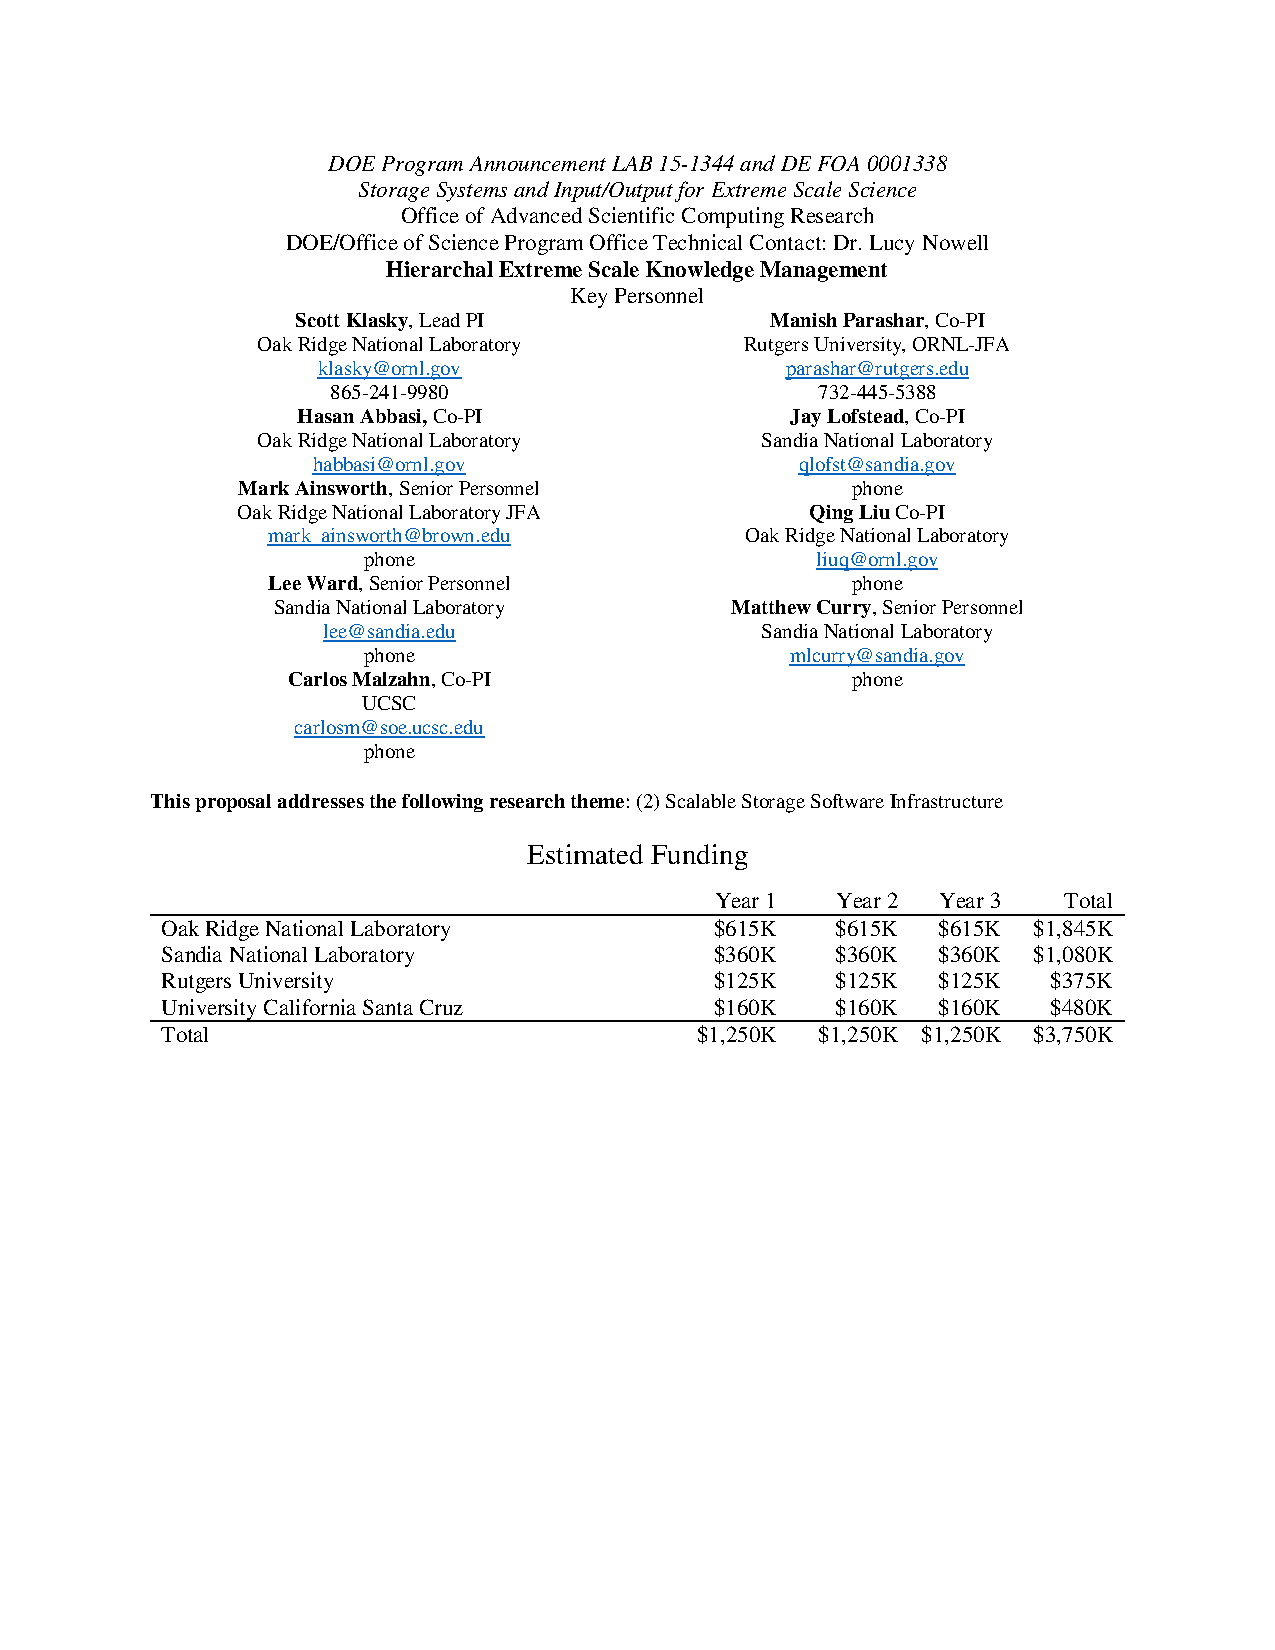
\includepdf[pages={1}]{ornl-cover.pdf}
  %  \pagebreak

\author{
  \IEEEauthorblockN {
    PI: Scott Klasky, % \IEEEauthorrefmark{1},
    Co-PI Manish Parashar % \IEEEauthorrefmark{1}
  }
  \IEEEauthorblockA {
    % \IEEEauthorrefmark{1}
    Mathematics and Computer Science Division,
    Argonne National Laboratory,
    Argonne, IL, USA}
}

%  \maketitle

  %  Heilmeyer Points: from http://www.csee.umbc.edu/~finin/home/heilmeyerCatechism.html
  %  
  %  \begin{enumerate}

  %  \item What is the problem, why is it hard? 

  %  \item How is it solved today?
  %    Fig A: much 

  %  \item What is the new technical idea; why can we succeed now?
  %    Integration of proven components into an architecture that solves
  %    problems. New research will resolve remaining technical hurdles.

  %  \item What is the impact if successful?
  %    Users and developers will be able to ...

  %  \item How will the program be organized?
  %    Participants and focus areas

  %  \item How will intermediate results be generated?
  %    Toolkit snapshots and application

  %  \item How will you measure progress?
  %    Provide metrics

  %  \item What will it cost?
  %    Cover sheet

  %  \end{enumerate}
  %   
\setlength{\parindent}{0cm}
{\bf Title of Pre-application:}  Extreme Scale Hierarchal Knowledge Management \par
{\bf Principal Investigator:} Scott Klasky, Group Leader, ORNL, 854-241-9980, klasky@ornl.gov \par
{\bf Funding Opportunity Announcement Number: DE-FOA-0001338} \par
 \vskip 0.0 in
\
\begin{tabular} {ll}
 \multicolumn{2}{l}{\bf Co-PIs and Key/Senior Personnel}\\
Hasan Abbasi, ORNL  & Mark Ainsworth, ORNL JFA, Brown University \\
Matthew Curry, SNL & Qing  Liu, ORNL \\
Jay Lofstead, ORNL & Kimmy Mu, ORNL \\
Carlos Malzahn, U. Cal. Santa Cruz & Manish Parashar, Rutgers University, ORNL \\
Feiyi Wang, ORNL & Lee Ward, SNL
\end{tabular}


\setlength{\parindent}{0.5cm}

\vskip 0.1 in


\underline{\textbf{Objectives:}} Exascale scientific discovery will be
severely bottlenecked without sufficient new research into managing and
storing the large amounts of data that will be produced during the
simulation, and analyzed for months afterwards.  Our goal in this project is
to address the associated I/O and storage challenges in the context of
current and emerging storage landscapes, and expedite insights into mission
critical scientific processes. To that end, we will build on the
capabilities offered by ADIOS and DataSpaces that provide I/O abstractions
and services, the Sirocco peer-to-peer file system at
Sandia and the object storage and annotation expertise of UC Santa Cruz, to
explore application and multi-tier storage aware data management
solutions.    This project
brings together a  team with strong expertise in I/O middleware (ORNL,
Rutgers), file system (SNL, UCSC) and storage (UCSC), and connect and
coordinate these key storage components in a seamless fashion.

Our solutions will provide novel functionalities and APIs for
\setlength{\parindent}{0cm}
1) specifying, at the application level, data annotations that enable the
qualification of the relative importance and utility of data objects, and
enable them to be mapped at runtime to appropriate storage capabilities
across the storage hierarchy;
%
2) specifying selectable performance/quality/cost tradeoffs from both the
application and system perspectives;
%
3) evaluating these tradeoffs at runtime during data placement and movement,
and executing the resultant policies in an autonomic system using models,
heuristics and continuous learning; and
%
4) leveraging techniques such as application-aware data compression, re-computation at the
requisite level of accuracy, and I/O prioritization to enforce these
policies.
%  2) a selectable performance/quality tradeoff when reading data, and
  %  the ability to recompute data if needed, and
  %  3) incorporate reader prioritization for data annotation, placement, and data
  %  quality when writing data.  
  
  \setlength{\parindent}{0.5cm}
  Our objective here is to reduce the time to knowledge, not just for a single
application or workflow, but for the entire workload in the system. This is
an end-to-end system wide metric relevant to the scientific discovery
process. We will explore beyond the traditional I/O pattern of
checkpoint/restart, and will address the challenges posed by other essential
data access patterns in the knowledge gathering process.  Through a deeper
insight into the scientific process we will encode and utilize accuracy and
errors as optimization parameters.  
Finally, we will take the knowledge from the storage system to provide vital feedback to the middleware 
so that the best possible decisions can be autonomically  between the user intentions and
the available system resources. Our overall goal is to ensure that optimizations can be made across
1) a single application, 2) an ensemble of applications, and 3) the entire suite of applications which are running on the system.


  \setlength{\parindent}{0.5cm}



%
Our objective here is to reduce the time to knowledge, not just for a single
application or workflow, but for the entire workload in the system. This is
an end-to-end system wide metric relevant to the scientific discovery
process. We will explore beyond the traditional high volume I/O pattern of
checkpoint/restart, and will address the challenges posed by other essential
data access patterns in the knowledge gathering process.  Through a deeper
insight into the scientific process we will encode and utilize accuracy and
errors as optimization parameters. 
Ultimately, we will take the knowledge from the storage system to provide vital feedback to the middleware 
so that the best possible decisions can be autonomically  between the user intentions and
the available system resources.  
We will test our prototypes  on current and future DOE system with many of today's applications, including the
s XGC1, GTC, QMCPack, and SpecFM3D simulations. 



 % For example, scientific simulations
%contain approximations, as do measurements from observations and
%experiments, and depending on the goal, these approximations are
%acceptable. We can leverage this observation to optimize the presentation of
%data to the user and to implement various tradeoffs -- users can ask for
%information within a given accuracy bound, allowing us to offer a tradeoff for
%re-computation vs. data storage and retrieval.




%  
% \TODO{\bf: please list other things from OLCF}
% 


\underline{\textbf{Key Technical Approach:}}

Our overall technical approach is based on an application-aware runtime
realization of tradeoffs in data representation, data placement and data
access. We will allow users plug-in their knowledge 
about the data, represented not as bytes but as motifs, allowing the I/O and 
storage system to understand user
intentions, the relationships between data objects, and also data access
and transport patterns. This will facilitate efficient mapping of data from
user space onto various storage tiers, and application-guided
data reductions.

%Our approach can be most easily understood by considering a traditional
%  supermarket logistics problem. Given a limited amount of shelf space,
%  fluctuating user demands and priorities, and the need to optimize profit at
%  a market wide level instead of per product, the logistical problem combines
%  predictions about the variants and the indicated constraints to find a
%  solution. Self space is itself not a homogenous, with different locations
%  providing greater rewards to the placed items. Furthermore, haphazard
%  organization of items produces suboptimal results because it would ignore
%  locality in purchasing. Backroom and warehouses represent tiers of storage
%  where objects can be stored in bulk, but have a substantial overhead (and
%  thus lower utility) in access. Similar to this scenario, the data management
%  problem is a complex logistics problem. Shelf space is analogous to high
%  performance/lower capacity storage. Locality is an important consideration,
%  not just for single data objects but also through the identification of
%  domain meaningful relationships between objects. The tiers of the storage
%  hierarchy provide lower cost for data storage, but also increase the
%  overhead for access.

Incorporating awareness of the data content and user intent  into
our decision making and data management process is integral to our approach. For example, 
we will offer a coarse grained, quick overview of a data set with progressively more detail in 
areas of interest such as those containing features, and less detail in areas
without. These progressively more detailed data views require more storage
space and time to retrieve. By defining mechanisms for applications to provide this 
knowledge and incorporating its awareness into our middleware  and storage allow
it will be able to selectively store data at different  levels, and allow a user to select what data to retrieve by specifying both an acceptable  timeframe and accuracy.

%The user may also specify guidelines that are funneled through the I/O middleware and 
%provide advice on how to react if the timeframe and error bound cannot be accepted.

%\hasan{Since we are laying the foundation for a real storage system we can't
%  be solving the problem for a single application. We will eventually have
%  to consider things like fairness, availability and this is also why we
%  want to tie in with the resource management system} 



The I/O and storage system prototype will enable
highly flexible data access modes that are common in scientific applications
and associated analysis.
%
%\hasan{Can we actually take some lower accuracy representation of data (low
%  granularity MR for example, and compute more stuff to provide a higher
%  accuracy representation? I am thinking of the work with Varis Carey with
%  storing boundary state instead of full volume and then using those
%  boundaries to fill in blanks over temporally changing data}
%
\textbf{First}, data re-computation is allowed to re-generate data with
customizable accuracy, if the associated computing and I/O cost is lower
than retrieving the target data from a {\em slow} tier.
%
\textbf{Second}, exploratory analysis operations frequently entail an
overall data set view followed by targeted data exploration on extracted
features.  In particular, the {\em overview} access mode gives a quick but
approximate data view that can guide feature selection offering rapid
coarse-grained data exploration without requiring loading the high-accuracy
data from storage. Based on the granularity requested, the accuracy and size
of the data returned can be adjusted. In the most extreme setting, the
original data can be retrieved at the time cost of moving the potentially
huge data quantity.
%
\textbf{Third}, to ensure available storage for subsequent operations, we
will offer automatic data migration, based on user annotations for required data and using monitoring and learning techniques.  Unlike existing approaches, this will be
driven both by the user annotations and through learned access patterns in
an autonomic and crosslayer manner.  While past access patterns may not
indicate future access because the simulation run purpose may have changed,
we are focused on scalability where subsequent runs are larger as the
simulation prepares for a capability run.  By learning from the output and
access patterns during this run sequence, we can accurately decide how to
place and organize data for the critical capability runs.
%
\textbf{Fourth}, we anticipate storing multiple data copies, each compressed
in different ways according to the underlying media, some of these copies
will disappear based on storage pressures, but data persistence will be
maintained according to user specifications. Assuming a relatively low
latency cache layer before a tape system, we can offer exploratory data
access reserving pulling data from tape to just the data required. 
 Additionally, we will incorporate data life time, at sub-object
granularity, as a user described metric to allow the storage system to
intelligently make decisions on purging and evicting data. 


A key challenge in this project is defining and maintaining the metadata
connecting different object quality and utility levels, and using this metadata 
to most appropriately manage the placement and access of data object based on 
user/application intent/constraints and storage system state.
%The new user APIs required to interact with this rich metadata system will
%drive effective use of the entire middleware and storage stack.
Our research efforts will be heavily focused on the need to, in a
coordinated manner, adapt data and metadata retention policies to the
dynamic resource balancing that will need to take place between the
application, OS/R, and hardware.

The success of this project will provide insights into how to build
autonomic middleware and storage layers which can interact well with each
other, and take user-provided hints.  This will be managed against the needs of
individual simulations as well as what's happening on the entire system. This
will reduce the time to knowledge by allowing user and system knowledge into
the SSIO software layers.

%Today, data is reduced by application
%scientist who have limited information on what the storage layer can
%provide. 

%They often make compromises based on this limited knowledge and
%either tune their output for writing or reading performance. This data then
%gets moved to other locations, and much of the tuning is lost when the data
%is read back during their post processing. Furthermore, there is a limited
%set of operations which users will be able to stage to other staging nodes
%for real-time-reduction and visualization.


%  \includepdf[pages={1}]{COI.pdf}

\end{document}

%%% End: 

%%% Local Variables:
%%% mode: latex
%%% TeX-master: t
%%% End:
